%!TEX root=/home/ska124/Dropbox/Thesis/thes-full.tex

%%%%%%%%%%%%%%%%%%%%%%%%%%%%%%%%%%%%%%%%%%%%%%%%%
%
%     Chapter 4   
%
%%%%%%%%%%%%%%%%%%%%%%%%%%%%%%%%%%%%%%%%%%%%%%%%

\chapter{Hardware Complexity and Simulation Infrastructure}
\label{chap:hardware_complexity_and_simulation}

This chapter describes the additional hardware complexity added to an \AC\ with respect to a conventional cache in order to support variable granularity \AB{}s. The chapter also describes the simulation infrastructure used to evaluate the performance of the \AC{}.

\section{Hardware Complexity}  
\label{sec:hardware_complexity}

The complexity of the \AC\ is analysed along the following directions:
\begin{itemize}
  \item Additional complexity of the cache controller
  \item Area, latency and energy overhead
  \item Challenges of megabyte sized \AC{}s
\end{itemize}


\subsection{Cache Controller} 

\begin{figure}[!h]
  \centering
  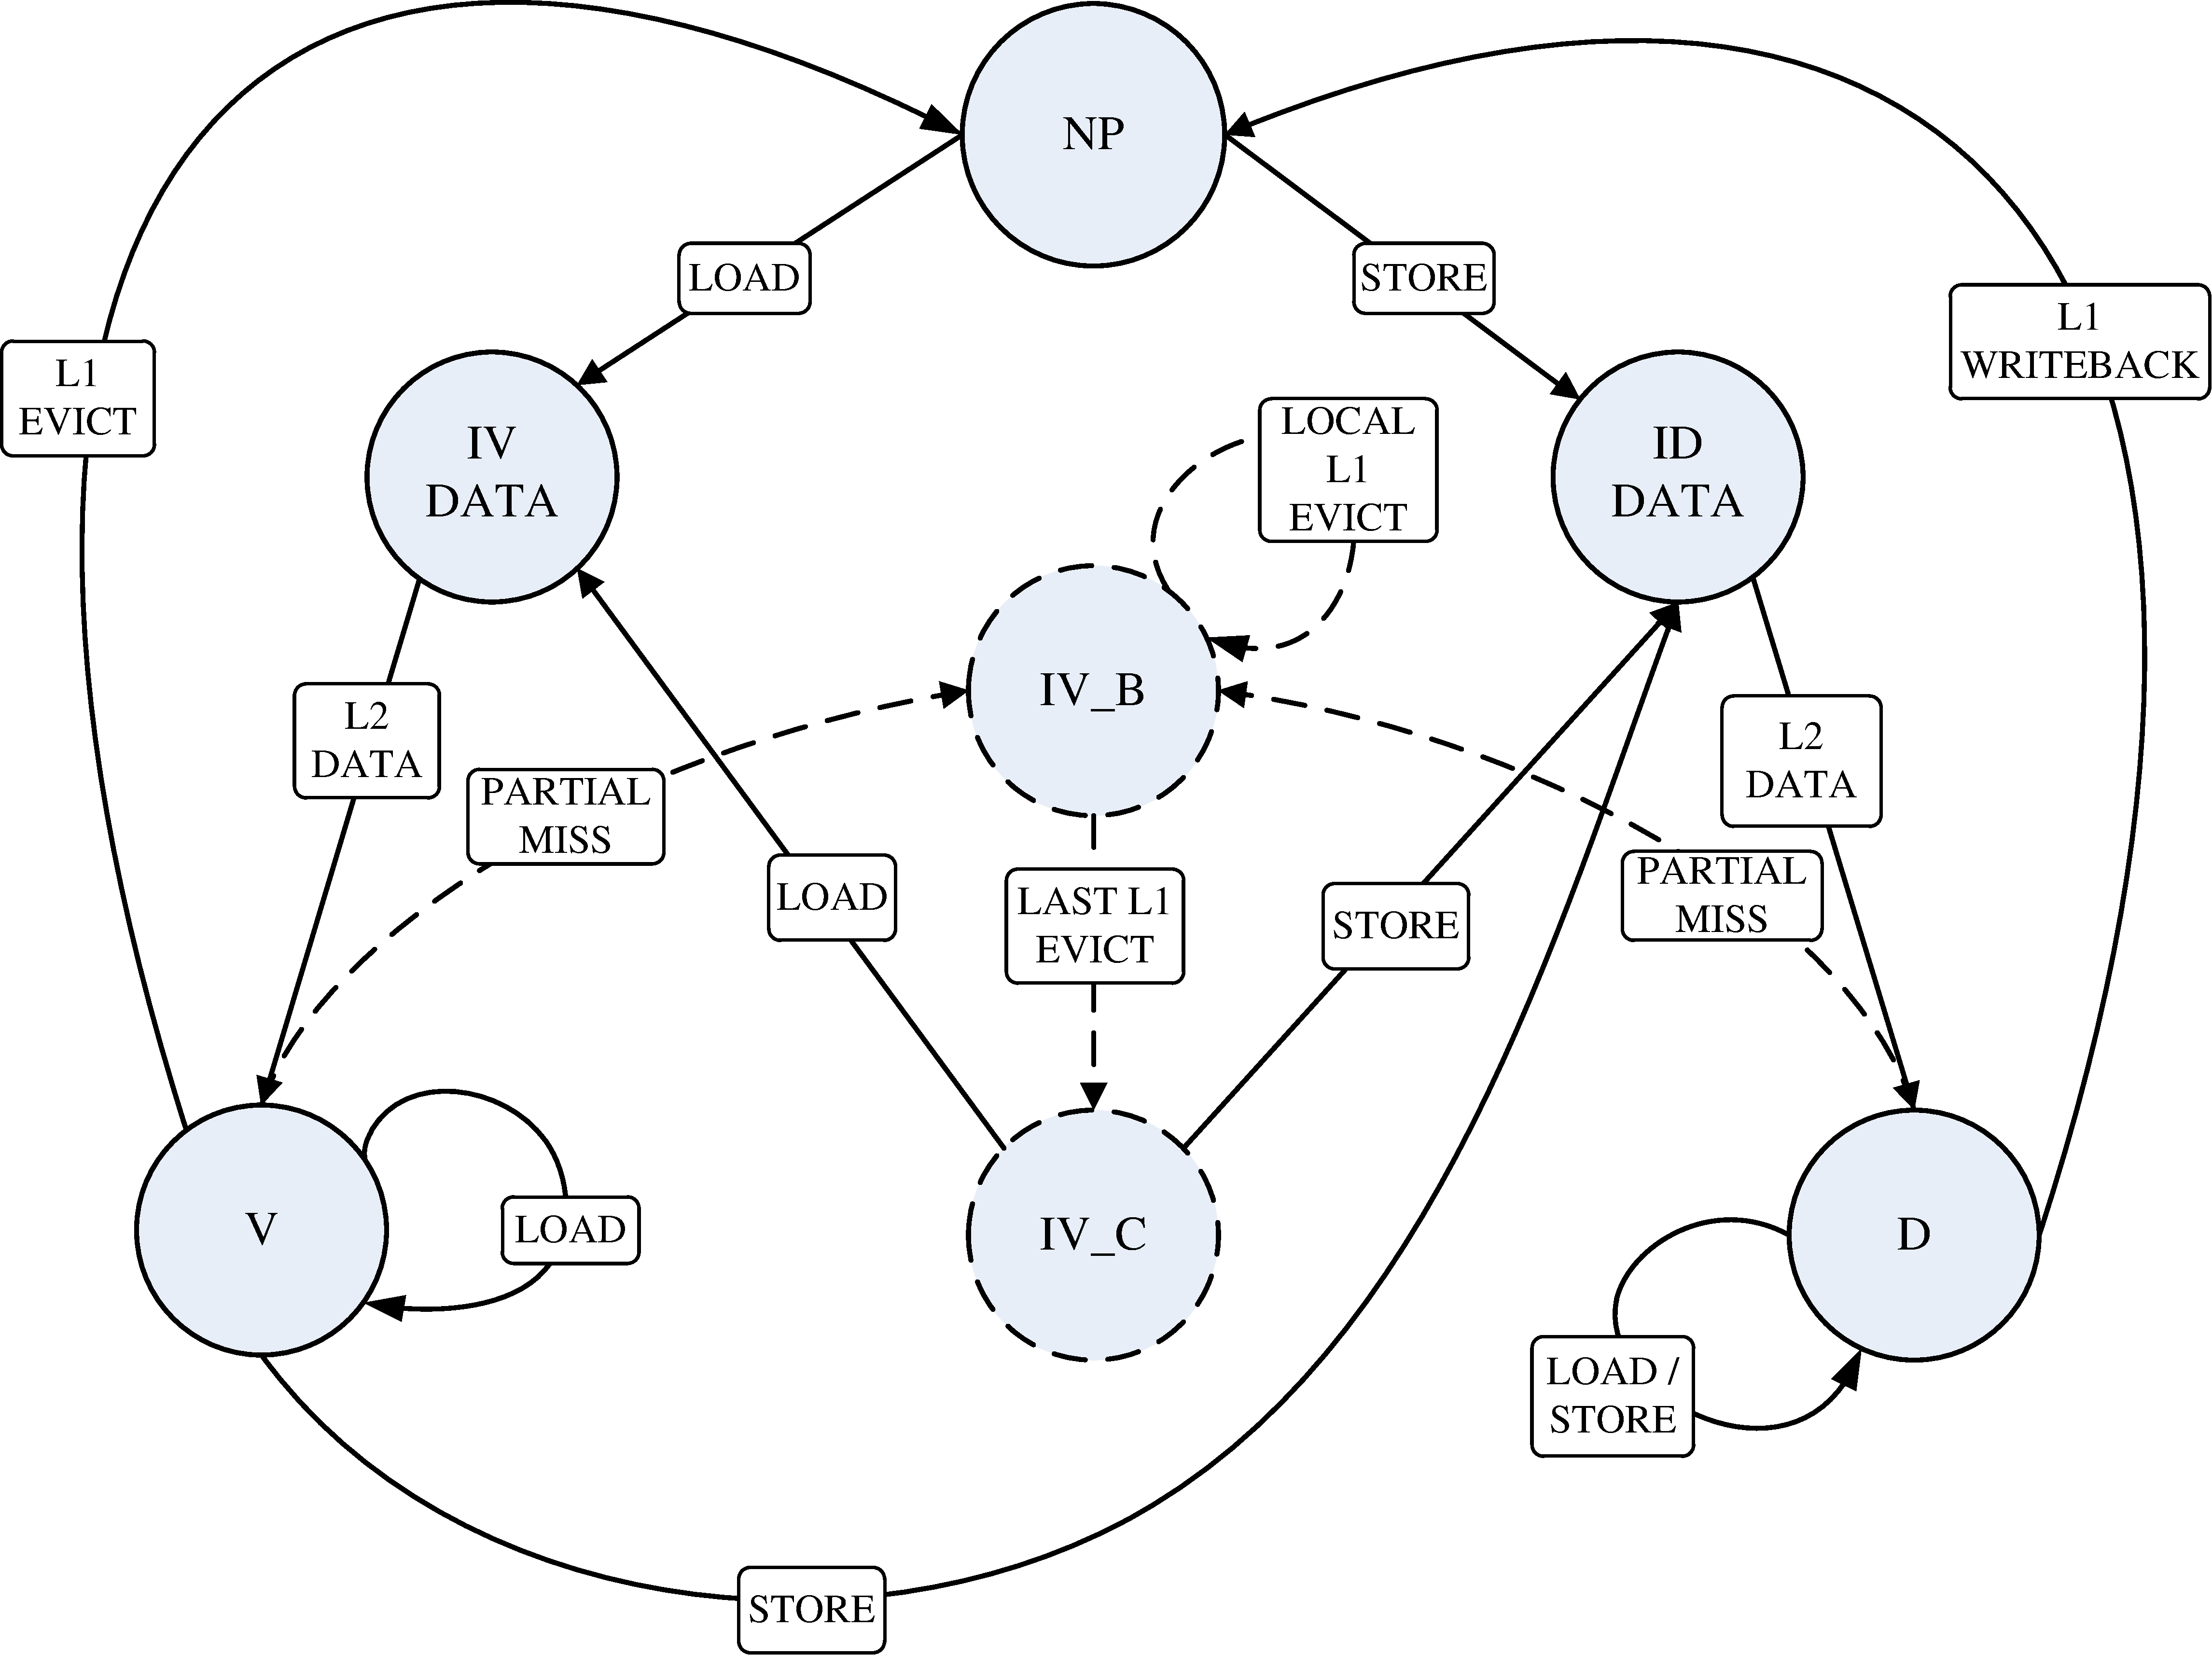
\includegraphics[width=\textwidth]{files/Figures/07-L1CC.pdf}
  \\ 
  \vspace{15pt}
  {
  \small
  \begin{tabular}{|@{~}c@{~}|@{~}p{0.75\textwidth}|} 
        
        \multicolumn{2}{c}{ \textbf{L1 cache controller states}}\\
        \hline
        State & Description \\
        \hline
        NP & \AB\ not present in the cache. \\
        \hline
        V & All words corresponding to \AB\ present and valid (read-only) \\
        \hline
        D & Valid and atleast one word in \AB\ is dirty (read-write) \\
        \hline
        {\bf IV\_B} & Partial miss being processed (blocking state) \\
        \hline
        {\bf IV\_Data} & Load miss; waiting for data from L2\\
        \hline
        ID\_Data & Store miss; waiting for data. Set dirty bit. \\
        \hline
        {\bf IV\_C} & Partial miss cleanup from cache completed (treat as full miss) \\ 
        \hline
        \multicolumn{2}{c}{}\\
        \multicolumn{2}{c}{ \textbf{ \AC\ specific events}}\\
        \hline
        \multicolumn{2}{|p{5in}|}{Partial miss: Process partial miss.} \\
        \multicolumn{2}{|p{5in}|}{Local\_L1\_Evict: Remove overlapping \AB\ to MSHR.} \\
        \multicolumn{2}{|p{5in}|}{Last\_L1\_Evict: Last \AB\ moved to MSHR. Convert to full miss and process load or store.} \\
        \hline
    \end{tabular}
    }
  \caption{\textbf{L1 Cache Controller for \AC\ } : The \AC\ specific states and events are marked by dashed lines. The \AC\ specific events are described in the table.}
  \label{fig:L1protocol}
\end{figure}

We focus on the L1 controller here, and in particular, partial misses. The cache controller manages operations at
the aligned RMAX granularity. The controller  permits only one in-flight cache operation per RMAX region. In-flight cache operations ensure no address overlap with stable  \AB{}s in order to eliminate complex race conditions. Figure~\ref{fig:L1protocol} shows the L1 cache controller state machine. We add two states to the default protocol, \code{IV\_B} and \code{IV\_C}, to handle partial misses. \code{IV\_B} is a blocking state that blocks other cache operations to RMAX region until all relevant \AB{}s to a partial miss are evicted (e.g., 0--3 and 5--7 blocks in Figure~\ref{fig:partial-miss}). \code{IV\_C} indicates partial miss completion. This enables the controller to treat the access as a full miss and issue the refill request. The other stable states (I, V, D) and transient states (\code{IV\_Data} and \code{ID\_Data}) are present in a conventional protocol as well. \code{Partial-miss} triggers the clean-up operations (\code{1} and \code{2} in Figure~\ref{fig:partial-miss}). \code{Local\_L1\_Evict} is a looping event that keeps retriggering for each \AB\ involved in the partial miss; \code{Last\_L1\_Evict} is triggered when the last \AB\ involved in the partial miss is evicted to the MSHR. A key difference between the L1 and lower-level protocols is that the Load/Store event in the lower-level protocol may need to access data from multiple \AB{}s. In such cases, similar to the partial-miss event, we read out each block independently before
supplying the data (more details in \S~\ref{sec:multicache}).


% \subsection{Area, Latency, and Energy Overhead}
% The extra metadata required by \AC\ are the T? (1 tag bit per word) and V? (1
% valid bit per word) bitmaps. Table~\ref{table:overheads} shows the quantitative
% overhead compared to the data storage. Both the T? and V?  bitmap
% arrays are directly proportional to the size of the cache and require a
% constant storage overhead (3\% in total). The T? bitmap is read in parallel
% with the data array and does not affect the critical path; T? adds 2\%---3.5\%
% (depending on cache size) to the overall cache access energy. 
% V? is referred only on misses when inserting a new block.

% \begin{table}[!htb]
% {
% \vspace{-10pt}
% \centering
% \caption{\AC\ Hardware Complexity.}
% \label{table:overheads}
% {
% \small 
% \begin{tabular}{|@{~}c@{~}|@{~}c@{~}|@{~}c@{~}|@{~}c@{~}|}
% \hline
% \multicolumn{4}{|c|}{Cache configuration}\\
% \hline
%              & 64K (256by/set) & 1MB (512by/set) & 4MB (1024by/set) \\
% \hline
% \multicolumn{4}{|l|}{Data RAM parameters} \\   
% \hline
% Delay        & 0.36ns & 2ns & 2.5 ns \\
% Energy       & 100pJ & 230pJ  & 280pJ \\
% \hline 
% \multicolumn{4}{|c|}{\AC\ components (CACTI model)} \\   
% \hline
% T?/V? map & 1KB &  16KB & 64KB \\
% Latency      & 0.019ns (5\%) & 0.12ns (6\%) & 0.2ns (6\%) \\   
% Energy       & 2pJ (2\%) & 8pJ (3.4\%) & 10pJ (3.5\%)  \\ 
% LRU  & $\frac{1}{8}$KB & 2KB & 8KB \\
% \hline
% \multicolumn{4}{|c|}{Lookup Overhead (VHDL model)} \\
% \hline
% Area    & 0.7\% & \multicolumn{2}{c|}{0.1\%} \\  
% \hline
% Latency & 0.02ns & 0.035ns & 0.04ns \\
% \hline
% \end{tabular}
% }

% {
%   \% indicates overhead compared to data array of cache. 64K cache operates in \textit{Fast mode}; 1MB and
%   4MB operate in \textit{Normal mode}. We use 32nm ITRS HP transistors for
%   64K and 32nm ITRS LOP transistors for 1MB and 4MB.
% }
% }
% \end{table}

% We synthesized\footnote{We do not have access to an industry-grade 32nm library, 
% so we synthesized at a higher 180nm node size and scaled the results to 32 nm 
% (latency and energy scaled proportional to Vdd (taken from~\cite{cpudb}) 
% and $Vdd^2$ respectively).}
%  the cache lookup logic using Synopsys and quantify the area,
% latency, and energy penalty. \AC\ is compatible with  \textit{Fast} and
% \textit{Normal} cache access modes~\cite[-access-mode config]{muralimanohar-
% micro-2007}, both of which read the entire set from the data array in parallel
% with the way selection to  achieve lower latency.  \textit{Fast} mode
% transfers the entire set to the edge of the H-tree, while  \textit{Normal}
% mode, only transmits the selected way over the H-tree. For synthesis, we used
% the Synopsys design compiler (Vision Z-2007.03-SP5).



% Figure~\ref{fig:Lookup} shows \AC\'s lookup hardware on the critical path; 
% we compare it
% against a fixed-granularity cache's lookup logic (mainly the comparators). The
% area overhead of the \AC\ includes registering an entire line that has been
% read out, the tag operation logic, and the word selector. The components on the
% critical path once the data is read out are the 2-way multiplexers, the $\in$
% comparators, and priority encoder that selects the word; the T?  bitmap is
% accessed in parallel and off the critical path. \AC\ is made feasible under
% today's wire-limited technology where the cache latency and energy is
% dominated by the bit/word lines, decoder, and H-tree~\cite{muralimanohar- micro-2007}.  \AC{}'s comparators, which operate on
% the entire cache set, are 6$\times$ the area of a fixed cache's comparators. 
% Note that the data array occupies 99\% of the overall cache area. The critical
% path is dominated by the wide word selector since the comparators all
% operate in parallel. The lookup logic adds 60\% to the conventional cache's
% comparator time. The overall critical path is dominated by the data array
% access and \AC{}'s lookup circuit adds 0.02ns to the access latency and
% $\simeq$ 1pJ to the energy of a 64K cache, and 0.035ns to the latency and
% $\simeq$2pJ to the energy of a 1MB cache. Finally, \AC\ amortizes the energy
% penalty of the peripheral components (H-tree, Wordline, and decoder) over a
% single RAM. 


% \REVIEW{\AC{}'s overhead needs careful consideration when implemented at the L1
% cache level. We have two options for handling the latency overhead a) if the L1
% cache is the critical stage in the pipeline, we can throttle the CPU clock by
% the latency overhead to ensure that the additional logic fits within the
% pipeline stage. This ensures that the number of pipeline stages for a memory
% access does not change with respect to a conventional cache, although all
% instructions bear the overhead of the reduced CPU clock. b) we can add an
% extra pipeline stage to the L1 hit path, adding a 1 cycle overhead to all
% memory accesses but ensuring no change in CPU frequency. We quantify the
% performance impact of both approaches in Section~\ref{sec:eval}.}


% \subsection{Tag-only Operations}  Conventional caches support tag-only
% operations to reduce data port contention. While the \AC\ merges tags and
% data, like many commercial processors it decouples the replacement metadata
% and valid bits from the tags, accessing the tags only on cache lookup. Lookups
% can be either CPU side or network side (coherence invalidation and
% Wback/Forwarding). CPU-side lookups and writebacks ($\simeq$ 95\% of cache
% operations) both need data and hence \AC\ in the common case does not
% introduce extra overhead. \AC\ does read out the entire data array unlike
% serial-mode caches (we discuss this issue in the next section). Invalidation
% checks and snoops can be more energy expensive with \AC{} compared to a
% conventional cache. Fortunately, coherence snoops are not common in many
% applications (e.g., 1/100 cache operations in SpecJBB) as a coherence
% directory and an inclusive LLC filter them out.


% \subsection{Tradeoff with Large Caches} \label{sec:extensions}
% \begin{figure}[!ht] \centering
% \begin{minipage}[c]{0.4\textwidth} {
% \includegraphics[width=\textwidth]{plots/predictors/Serial_vs_Normal.pdf}
% }
% \end{minipage}
% \begin{minipage}[c]{0.4\textwidth}
% {
% Baseline: Serial. $\leq1$ Normal is better.  32nm, ITRS  LOP.
% } 
% \end{minipage}  
% \caption{Serial vs Normal mode cache.}
% \label{fig:serial_parallel} 
% \end{figure}

% Large caches with many words per set ($\equiv$ highly associative conventional
% cache) need careful consideration.  \REVIEW{ Typically, highly associative
% caches tend to serialize tag and data access with only the relevant cache
% block read out on a hit and no data access on a miss. We first analyze the the
% tradeoff between reading the entire set (normal mode), which is compatible with
% \AC\, and only the relevant block (serial mode). } We vary the cache size from
% 2M---8M and associativity from 4(256B/set) --- 32 (2048B/set).  Under current
% technology constraints (Figure~\ref{fig:serial_parallel}), only at very high
% associativity does serial mode demonstrate a notable energy benefit. Large
% caches are dominated by H-tree energy consumption and reading out the entire
% set at each sub-bank imposes an energy penalty when bitlines and wordlines
% dominate (2KB+ \# of words/set).

% \begin{table}[!h]
% \begin{center}
% \vspace{-10pt}
% \caption{\% of direct accesses with fast tags}
% \label{fig:tagcount}
% {
% \small
% \begin{tabular}{|@{~}p{0.6in}@{~}|@{~}c@{~}|@{~}c@{~}|@{~}c@{~}|@{~}c@{~}|@{~}c@{~}|@{~}c@{~}|}
% \hline
% % \multicolumn{7}{|@{~}c@{~}|}{Cache Size}\\
%   &  \multicolumn{2}{@{~}c@{~}|} {64K(256by/set)} &  \multicolumn{2}{@{~}c@{~}|} {1MB(512by/set)} & \multicolumn{2}{@{~}c@{~}|} {2MB(1024 by/set)} \\
% \hline
% \# Tags/set &2 &  4 & 4 & 8 & 8 & 16 \\

% Overhead &  1KB & 2KB  & 2KB & 16KB  & 16KB & 32KB  \\  
% \hline
% {Benchmarks} & & & & & & \\

% Low      & 30\% & 45\% & 42\% & 64\% & 55\% & 74\%\\
% Moderate & 24\% & 62\% & 46\% & 70\% & 63\% & 85\%\\
% High     & 35\% & 79\% & 67\% & 95\% & 75\% & 96\%\\
% \hline
% \end{tabular}
% }
% \vspace{-10pt}
% \end{center}
% \end{table}


% \REVIEW{\AC\ can be tuned to minimize the hardware overhead for large caches.
% With many words/set the cache utilization improves due to longer block
% lifetimes making it feasible to support \AB{}s with a larger minimum
% granularity ($>$ 1 word). If we increase minimum granularity to two or four
% words, only every third or fifth word could be a tag, meaning the \# of
% comparators and multiplexers reduce to $\frac{N_{words/set}}{3}$ or
% $\frac{N_{words/set}}{5}$. When the minimum granularity is equal to max
% granularity (RMAX), we obtain a fixed granularity cache with
% $N_{words/set}/RMAX$ ways. Cache organizations that collocate all the tags
% together at the head of the data array enable tag-only operations and serial
% \AB\ accesses that need to activate only a portion of the data array. However, the set may need to be compacted at each insertion. Recently, Loh and Hill~\cite{loh- hill-micro-2011} explored such an organization for
% supporting tags in multi-gigabyte caches.}


% Finally, the use of \textit{Fast Tags} help reduce the tag lookups in the
% data array. Fast tags use a separate traditional tag array-like structure to
% cache the tags of the recently-used blocks and provide a pointer directly to
% the \AB{}. The \# of \textit{Fast Tags} needed per set is proportional to the
% \# of blocks in each set, which varies with the spatial locality in the
% application and the \# of bytes per set (more details in
% Section~\ref{sec:efficiency}). We studied 3 different cache configurations
% (64K 256B/set, 1M 512B/set, and 2M 1024B/set) while varying the number of 
% fast tags per set (see Table~\ref{fig:tagcount}). 
% With 8 tags/set (16KB
% overhead), we can filter 64---95\% of the accesses in a 1MB cache and 55---
% 75\% of the accesses in a 2MB cache.


\section{Simulation Infrastructure}

% \section{Application Traces}
% \subsection{Intel Pin}
% \subsection{Generating a memory access trace}
% \subsection{Workload selection}
% \section{GEMS Infrastructure}
% \subsection{Introduction}
% \subsection{Components}
% \subsection{SLICC}
% \subsection{Amoeba-Single Protocol}
